% =====================================================================
%  LAPORAN TUGAS AKHIR -- Bentuk 1: Penelitian Konvensional
%  Program Studi Teknik Informatika, Fakultas Teknologi Industri
%  Institut Teknologi Sumatera (ITERA)
%
%  Compiler Overleaf : pdfLaTeX (Menu > Settings > Compiler)
%  Daftar pustaka    : BibTeX, gaya IEEE (IEEEtran)
% =====================================================================
\documentclass[11pt,twoside,openany]{report}
\usepackage{itera-ta}

% ---------------------------------------------------------------------
%  SAKELAR TAHAP & PETUNJUK
% ---------------------------------------------------------------------
\sidangakhirtrue     % \sidangakhirfalse untuk naskah seminar proposal (Bab I-III)
\petunjuktrue        % \petunjukfalse untuk menyembunyikan semua teks "Petunjuk:"
\newif\iftampilpanduan
\tampilpanduantrue   % \tampilpanduanfalse untuk naskah final
                     % (menghapus halaman Petunjuk Pengisian & Peta Kewajiban)

% ---------------------------------------------------------------------
%  DATA TUGAS AKHIR -- ISI DI SINI, otomatis dipakai di semua halaman
% ---------------------------------------------------------------------
% Judul maksimal 16 kata, ditulis sama persis di semua halaman.
\newcommand{\judulTA}{\isian{Judul Tugas Akhir, maksimal 16 kata}}
% Judul yang sama dalam HURUF KAPITAL untuk sampul:
\newcommand{\judulTAkapital}{\isian{JUDUL TUGAS AKHIR: OBJEK, METODE, DAN KONTEKS PENELITIAN}}
\newcommand{\namaMhs}{\isian{Nama mahasiswa}}
\newcommand{\nimMhs}{\isian{NIM}}
\newcommand{\ttlMhs}{\isian{Tempat, tanggal lahir}}
\newcommand{\pembimbing}{\isian{Nama dan gelar}}
\newcommand{\nipPembimbing}{\isian{\dots\dots\dots\dots}}
\newcommand{\pengujiSatu}{\isian{Nama dan gelar}}
\newcommand{\nipPengujiSatu}{\isian{\dots\dots\dots\dots}}
\newcommand{\pengujiDua}{\isian{Nama dan gelar}}
\newcommand{\nipPengujiDua}{\isian{\dots\dots\dots\dots}}
\newcommand{\koorprodi}{\isian{Nama dan gelar}}
\newcommand{\nipKoorprodi}{\isian{\dots\dots\dots\dots}}
\newcommand{\tanggalTA}{\isian{tanggal}}
\newcommand{\tahunTA}{\isian{TAHUN}}
\newcommand{\pasfoto}{}  % isi: gambar/pasfoto.jpg (kosongkan bila belum ada)

\hypersetup{pdftitle={Laporan Tugas Akhir}, pdfauthor={Mahasiswa IF ITERA}}

\begin{document}

% =====================================================================
%  BAGIAN AWAL (nomor halaman romawi kecil)
% =====================================================================
\pagenumbering{roman}
% =====================================================================
%  HALAMAN SAMPUL
% =====================================================================
\begin{titlepage}
\centering
\singlespacing
\vspace*{0.3cm}
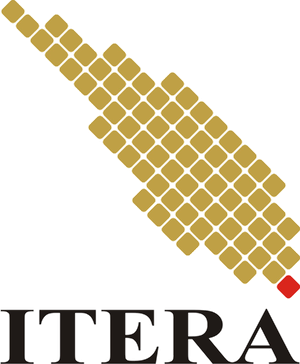
\includegraphics[width=2.4cm]{gambar/logo-itera.png}\par
\vspace{1cm}

{\bfseries\large TUGAS AKHIR\par}
{\bfseries\large LAPORAN TUGAS AKHIR\par}
{\small Bentuk 1: Penelitian Konvensional\par}
\vspace{1.2cm}

{\bfseries\fontsize{13}{16}\selectfont \judulTAkapital\par}
\ifpetunjuk{\scriptsize\itshape\color{abuisian}[Judul maksimal 16 kata]\par}\fi
\vspace{1.2cm}

{\small Diajukan sebagai luaran mata kuliah Tugas Akhir (IF25-40033)\par}
\vspace{1.2cm}

{\small\bfseries Disusun oleh:\par}
{\small \namaMhs\quad \nimMhs\par}
\vspace{0.6cm}
{\small Pembimbing: \pembimbing\par}

\vfill
{\small\bfseries
PROGRAM STUDI TEKNIK INFORMATIKA\par
FAKULTAS TEKNOLOGI INDUSTRI\par
INSTITUT TEKNOLOGI SUMATERA\par
LAMPUNG SELATAN\par}
{\small \tahunTA\par}
\vspace*{0.3cm}
\end{titlepage}

% =====================================================================
%  LEMBAR PENGESAHAN
% =====================================================================
\setcounter{page}{2}
\halaman{LEMBAR PENGESAHAN}
\enlargethispage{2\baselineskip}

\noindent Saya menyatakan bahwa Tugas Akhir berjudul ``\judulTA'' merupakan
hasil karya saya sendiri dan belum pernah diajukan, baik sebagian maupun
seluruhnya, di Institut Teknologi Sumatera atau institusi pendidikan lain
oleh saya maupun pihak lain.

\vspace{0.3cm}
\noindent
\begin{minipage}[t]{0.6\linewidth}
\singlespacing
Lampung Selatan, \tanggalTA\\[1.6cm]
\namaMhs\\
\nimMhs
\end{minipage}\hfill
\begin{minipage}[t]{3cm}
\vspace{0pt}
\ifdefempty{\pasfoto}
  {\fbox{\parbox[c][4cm][c]{2.8cm}{\centering\small\isian{Pas foto 3\texttimes4 berwarna}}}}
  {\includegraphics[width=3cm,height=4cm]{\pasfoto}}
\end{minipage}

\vspace{0.2cm}
{\singlespacing\small
\noindent Diperiksa dan disetujui oleh,\\[2pt]
\textbf{Pembimbing}
\begin{enumerate}[label=\arabic*., leftmargin=1.5em]
  \item \pembimbing\\[0.45cm] NIP. \nipPembimbing
\end{enumerate}
\vspace{4pt}
\noindent\textbf{Penguji}
\begin{enumerate}[label=\arabic*., leftmargin=1.5em]
  \item \pengujiSatu\\[0.45cm] NIP. \nipPengujiSatu
  \item \pengujiDua\\[0.45cm] NIP. \nipPengujiDua
\end{enumerate}

\vspace{-0.2cm}
\begin{center}
Disahkan oleh,\\
Koordinator Program Studi Teknik Informatika\\
Fakultas Teknologi Industri\\
Institut Teknologi Sumatera\\[1.0cm]
\koorprodi\\
NIP. \nipKoorprodi
\end{center}}
\clearpage

% =====================================================================
%  HALAMAN PERNYATAAN ORISINALITAS
% =====================================================================
\halaman{HALAMAN PERNYATAAN ORISINALITAS}

\noindent Yang bertanda tangan di bawah ini:

\begin{tabular}{@{}p{3.6cm}@{\,:\,}p{6cm}@{}}
\normalsize Nama               & \normalsize \namaMhs \\
\normalsize NIM                & \normalsize \nimMhs \\
\normalsize Tempat, tgl. lahir & \normalsize \ttlMhs \\
\normalsize Program studi      & \normalsize Teknik Informatika \\
\normalsize Fakultas           & \normalsize Teknologi Industri \\
\normalsize Judul Tugas Akhir  & \normalsize \judulTA \\
\end{tabular}

\vspace{0.3cm}
\noindent menyatakan dengan sesungguhnya bahwa Tugas Akhir dengan judul
tersebut di atas adalah benar-benar hasil karya saya sendiri, bukan merupakan
duplikasi atau plagiasi dari karya orang lain, dan belum pernah diajukan untuk
memperoleh gelar kesarjanaan di perguruan tinggi mana pun. Seluruh sumber yang
dikutip maupun dirujuk telah saya nyatakan dengan benar dalam naskah Tugas
Akhir ini.

Apabila di kemudian hari terbukti terdapat penyimpangan atau ketidakbenaran
dalam pernyataan ini, saya bersedia menerima sanksi akademik sesuai dengan
peraturan yang berlaku di Institut Teknologi Sumatera, termasuk pencabutan
gelar kesarjanaan yang telah saya peroleh.

\vspace{0.5cm}
\begin{flushright}
\singlespacing
\begin{tabular}{c}
\normalsize Lampung Selatan, \tanggalTA\\
\normalsize Yang membuat pernyataan,\\[0.8cm]
\normalsize\isian{Materai Rp10.000}\\[0.8cm]
\normalsize (\namaMhs)\\
\normalsize NIM. \nimMhs
\end{tabular}
\end{flushright}
\clearpage

\ifsidangakhir % =====================================================================
%  HALAMAN PERNYATAAN PENGGUNAAN KECERDASAN ARTIFISIAL (AI)
%  Wajib pada sidang akhir (Pedoman TA Bab 4.2.1, Lampiran 2)
% =====================================================================
\halaman{HALAMAN PERNYATAAN PENGGUNAAN KECERDASAN ARTIFISIAL (AI)}

\petunjuk{Wajib diisi pada laporan sidang akhir, termasuk bila tidak memakai
AI (Pedoman TA Bab 4.2.1, Lampiran 2). Untuk TA kelompok, setiap anggota
mengisi satu halaman ini. Lampirkan log sesi AI dan riwayat versi laporan
serta kode. \tahap{\TidakPerlu}{\WAJIB}}

\noindent Yang bertanda tangan di bawah ini:

\begin{tabular}{@{}p{3.6cm}@{\,:\,}p{6cm}@{}}
\normalsize Nama              & \normalsize \namaMhs \\
\normalsize NIM               & \normalsize \nimMhs \\
\normalsize Program studi     & \normalsize Teknik Informatika \\
\normalsize Judul Tugas Akhir & \normalsize \judulTA \\
\end{tabular}

\vspace{0.2cm}
\noindent menyatakan dengan sesungguhnya bahwa dalam proses penyusunan Tugas
Akhir ini, saya:

% Ganti \kotak menjadi \kotakcentang pada pilihan yang sesuai
\begin{itemize}[label={}, leftmargin=0pt]
  \item \kotak\ \textbf{TIDAK} menggunakan alat bantu Kecerdasan Artifisial (AI)
        dalam bentuk apa pun.
  \item \kotak\ \textbf{MENGGUNAKAN} alat bantu Kecerdasan Artifisial (AI)
        dengan rincian pada tabel berikut.
\end{itemize}

\begin{center}
\renewcommand{\arraystretch}{1.4}
\begin{tabularx}{\linewidth}{|c|X|X|X|X|}
\hline
\rowcolor{bgkepala}
\textbf{No} & \textbf{Nama AI dan versi} & \textbf{Tujuan} &
\textbf{Bagian TA} & \textbf{Verifikasi} \\ \hline
1 & & & & \\ \hline
2 & & & & \\ \hline
3 & & & & \\ \hline
\end{tabularx}
\end{center}

\noindent Saya menyadari dan bertanggung jawab penuh bahwa:
\begin{enumerate}[leftmargin=1.5em]
  \item Seluruh isi Tugas Akhir, termasuk bagian yang dibantu AI, merupakan
        tanggung jawab saya sepenuhnya.
  \item Setiap fakta, referensi, dan data yang diperoleh dari AI telah saya
        verifikasi kebenarannya.
  \item Saya mampu menjelaskan seluruh bagian Tugas Akhir secara lisan,
        termasuk \textit{code walkthrough}.
  \item Apabila ditemukan ketidakjujuran dalam pernyataan ini, saya bersedia
        menerima sanksi akademik sesuai Peraturan Rektor ITERA Nomor 10 Tahun
        2025.
\end{enumerate}

\vspace{0.4cm}
\begin{flushright}
\singlespacing
\begin{tabular}{c}
\normalsize Lampung Selatan, \tanggalTA\\
\normalsize Yang membuat pernyataan,\\[1.8cm]
\normalsize (\namaMhs)\\
\normalsize NIM. \nimMhs
\end{tabular}
\end{flushright}
\clearpage
 \fi
\iftampilpanduan
  % =====================================================================
%  PETUNJUK PENGISIAN  (HAPUS DARI NASKAH FINAL: \tampilpanduanfalse)
% =====================================================================
\halaman{PETUNJUK PENGISIAN}

{\itshape
\noindent Halaman ini dan halaman Peta Kewajiban dihapus dari naskah final
(atur {\upshape\texttt{\textbackslash tampilpanduanfalse}} di \texttt{main.tex}). Isi
setiap bab dan subbab dalam bentuk paragraf. Teks miring berawalan
``Petunjuk:'' menjelaskan isi yang diharapkan dan harus dihapus setelah bagian
itu ditulis (atau sembunyikan seluruhnya dengan
{\upshape\texttt{\textbackslash petunjukfalse}}); teks abu-abu dalam kurung siku diganti
dengan isi Anda.

Tabel hanya dipakai untuk menyajikan data yang memang berbentuk tabel, diberi
nomor dan judul (Tabel 2.1 di atas tabel), dan dirujuk dalam narasi. Jangan
menulis isi bab atau subbab di dalam tabel atau kotak.\par}

\begin{itemize}[label=\textbullet, leftmargin=1.2em, itemsep=2pt]
  \item Judul penelitian maksimal 16 kata dan ditulis sama persis di sampul,
        lembar pengesahan, pernyataan, dan presentasi.
  \item Pengerjaan bersifat individu. Topik boleh beririsan dengan payung riset
        dosen, tetapi kontribusi orisinal Anda harus dapat dibedakan (Pedoman
        TA 3.1.2).
  \item Naskah seminar proposal berisi Bab I sampai III; laporan sidang akhir
        berisi Bab I sampai V lengkap. Lihat Peta Kewajiban.
  \item Ukuran naskah UNESCO (lebar 15,5 cm $\times$ tinggi 23 cm), Times New
        Roman 11 pt, spasi 1,5 (spasi 1 untuk abstrak, isi tabel, dan daftar
        pustaka), rata kiri-kanan (\textit{justify}). Margin atas 2 cm, kiri
        2,5 cm, bawah 2 cm, kanan 2 cm; dicetak bolak-balik dengan margin
        cermin (margin 2,5 cm selalu di sisi jilid). Judul tabel di atas tabel
        dan judul gambar di bawah gambar.
  \item Sitasi gaya IEEE; minimal 15 sumber, minimal 70\% terbit dalam 3 tahun
        terakhir; prioritaskan jurnal dan prosiding bereputasi (Pedoman TA 8.7).
  \item Kode sumber dikelola di git dengan \textit{commit} berkala (minimal
        mingguan); laporan dikerjakan dengan riwayat versi (Overleaf, Google
        Docs, atau \textit{Track Changes}). Akses diberikan ke pembimbing sejak
        awal dan ke penguji saat sidang (Pedoman TA 4.2.2).
  \item \textit{Code walkthrough} WAJIB pada sidang akhir bila TA memuat
        implementasi perangkat lunak. Siapkan Peta Kode pada Lampiran 4.
  \item \textit{Similarity} maksimal 25\% dan kutipan langsung maksimal 10\%
        (laporan Turnitin lengkap); Halaman Pernyataan AI wajib diisi (Pedoman
        TA 5.7, 4.2.1).
  \item Bimbingan minimal 4 kali per semester, dicatat di Form Kendali
        Bimbingan atau Kartu Kendali TASYS.
\end{itemize}

\subsection*{Cara penilaian}
\noindent\textbf{Seminar proposal.} Kualitas proposal 40\%, presentasi dan
tanya jawab 30\%, proses bimbingan 30\% (Tabel 5.7). Grade minimum B (65).

\noindent\textbf{Sidang akhir.} Kualitas laporan 30\%, presentasi dan
pertahanan 20\%, \textit{code walkthrough} 10\%, proses bimbingan 20\%,
orisinalitas dan kontribusi 20\% (Tabel 5.8). Grade minimum B (65).

\noindent\textbf{Kualitas laporan.} Dinilai dengan rubrik detail Tabel 5.9:
sistematika dan penulisan, pendahuluan, tinjauan pustaka, metodologi, hasil
dan pembahasan, kesimpulan dan saran.
\clearpage

  % =====================================================================
%  PETA KEWAJIBAN PER TAHAP  (HAPUS DARI NASKAH FINAL)
% =====================================================================
\halaman{PETA KEWAJIBAN PER TAHAP}

{\itshape\noindent Seminar proposal (TA 1): dilaksanakan sebelum penelitian;
yang dinilai adalah kelayakan rencana penelitian (Bab I sampai III). Sidang
akhir (TA 2): dilaksanakan setelah penelitian selesai; yang dinilai adalah
hasil, pembahasan, dan pemahaman mahasiswa.\par}

\vspace{0.2cm}
{\small\singlespacing\noindent \WAJIB: harus ada.
\textcolor{merahwajib}{\textbf{WAJIB bila berlaku}}: bila kondisinya terpenuhi.
\Opsional: boleh dikosongkan. \TidakPerlu: tidak diisi.\par}

% Makro sel berwarna
\newcommand{\cW}[1][WAJIB]{\cellcolor{bgwajib}\textcolor{merahwajib}{\textbf{#1}}}
\newcommand{\cO}{\cellcolor{bgops}\textcolor{kuningops}{\textbf{Opsional}}}
\newcommand{\cT}{\cellcolor{bgtidak}\textcolor{abuisian}{Tidak diperlukan}}

\vspace{0.3cm}
{\footnotesize
\renewcommand{\arraystretch}{1.15}
\setlength{\tabcolsep}{4pt}
\begin{longtable}{|>{\raggedright\arraybackslash}p{5.1cm}|
                   >{\centering\arraybackslash}p{2.45cm}|
                   >{\centering\arraybackslash}p{2.45cm}|}
\hline
\rowcolor{bgkepala}
\textbf{Bagian} & \textbf{Seminar proposal} & \textbf{Sidang akhir} \\ \hline
\endhead
Halaman judul, pengesahan, orisinalitas & \cW & \cW \\ \hline
Pernyataan penggunaan AI                & \cT & \cW \\ \hline
Kata pengantar                          & \cO & \cW \\ \hline
\textit{Abstract} dan Abstrak           & \cO & \cW \\ \hline
BAB I Pendahuluan                       & \cW & \cW[WAJIB (final)] \\ \hline
BAB II Tinjauan Pustaka                 & \cW & \cW[WAJIB (final)] \\ \hline
BAB III Metodologi                      & \cW & \cW[WAJIB (final)] \\ \hline
BAB IV Hasil dan Pembahasan             & \cT & \cW \\ \hline
BAB V Kesimpulan dan Saran              & \cT & \cW \\ \hline
Daftar pustaka                          & \cW & \cW \\ \hline
Lampiran 1 (Form Kendali Bimbingan)     & \cW & \cW \\ \hline
Lampiran 2 (berita acara seminar proposal) & \cT & \cW \\ \hline
Lampiran 3 sampai 5 (kode, peta kode, data) & \cO & \cW \\ \hline
Lampiran 6 sampai 8 (\textit{similarity}, log AI, riwayat versi) & \cT & \cW \\ \hline
Lampiran 9 (daftar riwayat hidup)       & \cT & \cO \\ \hline
\end{longtable}}

{\scriptsize\itshape\color{abuisian}\noindent Pembagian ini disusun dari
Pedoman TA Prodi IF dan rubrik TA non-konvensional; konfirmasikan ke
Koordinator TA bila ragu.\par}
\clearpage

\fi
% =====================================================================
%  KATA PENGANTAR
% =====================================================================
\halaman[toc]{KATA PENGANTAR}

\petunjuk{Ucapan syukur, tujuan penulisan, dan terima kasih kepada pihak yang
membantu. Maksimal 1 halaman. \tahap{\Opsional}{\WAJIB}}

\isian{Tulis kata pengantar di sini \dots}

\vspace{1cm}
\begin{flushright}
\singlespacing
\begin{tabular}{c}
Lampung Selatan, \tanggalTA\\[1.5cm]
\namaMhs
\end{tabular}
\end{flushright}
\clearpage

% =====================================================================
%  ABSTRACT (Bahasa Inggris, spasi 1)
% =====================================================================
\halaman[toc]{ABSTRACT}

\petunjuk{Bahasa Inggris, satu paragraf 150--250 kata, spasi 1: latar
belakang dan masalah, tujuan, metode (data, model, pembanding, metrik), hasil
utama dengan angka, dan kesimpulan. Tutup dengan 3--5 \textit{keywords}.
\tahap{\Opsional}{\WAJIB}}

\begin{singlespace}
\noindent\textit{\isian{Write the abstract here \dots}}

\vspace{0.4cm}
\noindent\textbf{\textit{Keywords:}} \textit{\isian{keyword 1; keyword 2;
keyword 3}}
\end{singlespace}
\clearpage

% =====================================================================
%  ABSTRAK (Bahasa Indonesia, spasi 1)
% =====================================================================
\halaman[toc]{ABSTRAK}

\petunjuk{Versi bahasa Indonesia dari \textit{Abstract}, isi setara,
150--250 kata, dilengkapi 3--5 kata kunci. \tahap{\Opsional}{\WAJIB}}

\begin{singlespace}
\noindent\isian{Tulis abstrak di sini \dots}

\vspace{0.4cm}
\noindent\textbf{Kata kunci:} \isian{kata kunci 1; kata kunci 2; kata kunci 3}
\end{singlespace}
\clearpage


\cleardoublepage
\phantomsection\addcontentsline{toc}{chapter}{DAFTAR ISI}
\tableofcontents
\clearpage
\phantomsection\addcontentsline{toc}{chapter}{DAFTAR TABEL}
\listoftables
\clearpage
\phantomsection\addcontentsline{toc}{chapter}{DAFTAR GAMBAR}
\listoffigures
% =====================================================================
%  DAFTAR SIMBOL DAN SINGKATAN (hapus \input-nya di main.tex bila tidak ada)
% =====================================================================
\clearpage
\halaman[toc]{DAFTAR SIMBOL DAN SINGKATAN}

\petunjuk{Daftar simbol dan singkatan beserta artinya, urut abjad. Hapus
halaman ini bila tidak ada.}

\begin{longtable}{@{}p{2.8cm}p{7.5cm}@{}}
\textbf{Simbol/Singkatan} & \textbf{Arti} \\ \hline
\endhead
AI   & \textit{Artificial Intelligence} (Kecerdasan Artifisial) \\
IEEE & \textit{Institute of Electrical and Electronics Engineers} \\
\isian{\dots} & \isian{\dots} \\
\end{longtable}


% =====================================================================
%  BAGIAN INTI (nomor halaman arab)
% =====================================================================
\cleardoublepage
\pagenumbering{arabic}
% =====================================================================
%  BAB I PENDAHULUAN
% =====================================================================
\chapter{PENDAHULUAN}
\label{bab:pendahuluan}

\petunjuk{Argumentasi ilmiah yang melatarbelakangi penelitian, arah
penelitian, dan batasannya (Pedoman TA 7.1). \tahap{\WAJIB}{\WAJIB{} (final)}}

\section{Latar Belakang}
\petunjuk{Mulai dari masalah umum di bidang Teknik Informatika lalu mengerucut
ke masalah spesifik. Tunjukkan kesenjangan antara kondisi yang diharapkan dan
kondisi aktual. Wajib didukung data empiris dan rujukan terkini
($\leq$5 tahun).}

\isian{Tulis uraian dalam bentuk paragraf.} Contoh sitasi IEEE: \cite{contoh2024jurnal}.

\section{Rumusan Masalah}
\petunjuk{Pertanyaan penelitian yang jelas, spesifik, terukur, dan dapat
dijawab dengan metode ilmiah. Contoh: Bagaimana kinerja algoritma X
dibandingkan Y pada dataset Z dalam hal akurasi dan waktu eksekusi?}

\begin{enumerate}[leftmargin=1.5em]
  \item \isian{\dots\dots\dots}
  \item \isian{\dots\dots\dots}
\end{enumerate}

\section{Tujuan Penelitian}
\petunjuk{Satu tujuan untuk setiap rumusan masalah; gunakan kata kerja
operasional (menganalisis, merancang, membandingkan, mengevaluasi).
Cantumkan indikator keberhasilan. Uraikan tujuan dan indikator keberhasilan
untuk setiap rumusan masalah.}

\isian{Tulis uraian dalam bentuk paragraf.}

\section{Batasan Penelitian}
\petunjuk{Jenis dan ukuran dataset, platform atau lingkungan eksperimen,
metrik evaluasi, dan hal yang tidak dicakup.}

\isian{Tulis uraian dalam bentuk paragraf.}

\section{Manfaat Penelitian}
\petunjuk{Manfaat teoritis (keilmuan) dan praktis (aplikasi nyata), realistis
dan selaras dengan luaran.}

\isian{Tulis uraian dalam bentuk paragraf.}

\section{Sistematika Penulisan}
\petunjuk{Satu paragraf pendek per bab yang merangkum isi Bab I sampai Bab V.}

\isian{Tulis uraian dalam bentuk paragraf.}

% =====================================================================
%  BAB II TINJAUAN PUSTAKA
% =====================================================================
\chapter{TINJAUAN PUSTAKA}
\label{bab:tinjauan}

\petunjuk{Analisis kritis terhadap literatur, bukan rangkuman sumber (Pedoman
TA 7.2). \tahap{\WAJIB}{\WAJIB{} (final)}}

\section{Landasan Teori}
\petunjuk{Konsep fundamental yang dipakai: definisi, prinsip kerja algoritma,
arsitektur, paradigma. Proporsional dengan kebutuhan penelitian; tambahkan
subbab 2.1.1, 2.1.2, dst.\ sesuai kebutuhan.}

\isian{Tulis uraian dalam bentuk paragraf.}

% \subsection{Konsep A}
% \subsection{Konsep B}

\section{Penelitian Terdahulu (\textit{State of the Art})}
\petunjuk{Bahas penelitian sebelumnya secara naratif dan kritis, lalu ringkas
dalam tabel perbandingan seperti contoh Tabel~\ref{tab:penelitian-terdahulu}
(pedoman 7.2.2). Tabel hanya ringkasan; analisis tetap ditulis dalam
paragraf.}

\isian{Tulis uraian naratif dan kritis, lalu rujuk
Tabel~\ref{tab:penelitian-terdahulu}.}

\begin{table}[H]
\caption{Perbandingan Penelitian Terdahulu}
\label{tab:penelitian-terdahulu}
\renewcommand{\arraystretch}{1.5}
\begin{tabularx}{\linewidth}{|>{\raggedright\arraybackslash}p{2.1cm}|X|X|X|}
\hline
\rowcolor{bgkepala}
\textbf{Peneliti (tahun)} & \textbf{Metode dan dataset} &
\textbf{Hasil utama} & \textbf{Keterbatasan} \\ \hline
 & & & \\ \hline
 & & & \\ \hline
 & & & \\ \hline
 & & & \\ \hline
\end{tabularx}
\end{table}

\isian{Paragraf ringkasan kesenjangan: apa yang belum dijawab penelitian
terdahulu dan bagaimana penelitian ini mengisinya.}

\section{Kerangka Pemikiran}
\petunjuk{Alur logika yang menjembatani teori dan metodologi; sisipkan
diagram blok atau \textit{flowchart}.}

\isian{Uraikan kerangka pemikiran dan rujuk
Gambar~\ref{fig:kerangka}.}

\begin{figure}[H]
\centering
% Ganti kotak berikut dengan: \includegraphics[width=0.9\linewidth]{gambar/kerangka-pemikiran.png}
\fbox{\parbox[c][4cm][c]{0.85\linewidth}{\centering
  \isian{Sisipkan diagram kerangka pemikiran}}}
\caption{Kerangka Pemikiran Penelitian}
\label{fig:kerangka}
\end{figure}

% =====================================================================
%  BAB III METODOLOGI
% =====================================================================
\chapter{METODOLOGI}
\label{bab:metodologi}

\petunjuk{Cara penelitian dilakukan, cukup rinci agar dapat direplikasi
(Pedoman TA 7.3). \tahap{\WAJIB}{\WAJIB{} (final)}}

\section{Alur Penelitian}
\petunjuk{Diagram alir tahapan (studi literatur, pengumpulan data,
perancangan, implementasi, pengujian, analisis) dan penjelasan naratif tiap
tahap.}

\begin{figure}[H]
\centering
% Ganti kotak berikut dengan: \includegraphics[width=0.8\linewidth]{gambar/alur-penelitian.png}
\fbox{\parbox[c][5cm][c]{0.7\linewidth}{\centering
  \isian{Sisipkan diagram alir penelitian}}}
\caption{Diagram Alir Penelitian}
\label{fig:alur-penelitian}
\end{figure}

\isian{Narasi tiap tahap pada Gambar~\ref{fig:alur-penelitian}.}

\section{Pengumpulan Data}
\petunjuk{Sumber data, karakteristik, metode pengumpulan, praproses, dan
pembagian data latih/validasi/uji tanpa kebocoran data. Sertakan izin, etika,
dan anonimisasi bila memakai data pribadi (UU No.~27 Tahun 2022). Uraikan
secara naratif: sumber dan lisensi/izin, jumlah sampel dan atribut, metode
pengumpulan, praproses, dan pembagian data.}

\isian{Tulis uraian dalam bentuk paragraf.}

\section{Perancangan Sistem/Model}
\petunjuk{Arsitektur, pemilihan algoritma beserta justifikasi, hiperparameter,
dan spesifikasi teknis. Untuk perangkat lunak sertakan UML (\textit{use case},
\textit{class}, \textit{sequence}) atau DFD.}

\isian{Tulis uraian dalam bentuk paragraf.}

\section{Lingkungan Eksperimen}
\petunjuk{Wajib untuk reprodusibilitas. Uraikan secara naratif: CPU / GPU /
RAM, sistem operasi, bahasa pemrograman dan versi, \textit{framework/library}
dan versi, platform \textit{cloud} (bila ada), \textit{seed} acak, dan
repositori kode.}

\isian{Tulis uraian dalam bentuk paragraf.}

\section{Metode Pengujian dan Evaluasi}
\petunjuk{Metrik evaluasi beserta rumus (nomor persamaan rata kanan) dan
skenario uji, misalnya \textit{k-fold cross-validation}, uji pada dataset
terpisah, \textit{stress test}, atau uji usabilitas.}

\isian{Tulis uraian dalam bentuk paragraf.} Contoh penulisan persamaan
bernomor seperti Persamaan~\eqref{eq:akurasi}:
\begin{equation}
  \text{Akurasi} = \frac{TP + TN}{TP + TN + FP + FN}
  \label{eq:akurasi}
\end{equation}
dengan $TP$, $TN$, $FP$, dan $FN$ berturut-turut menyatakan
\textit{true positive}, \textit{true negative}, \textit{false positive}, dan
\textit{false negative}.

\ifsidangakhir
  % =====================================================================
%  BAB IV HASIL DAN PEMBAHASAN  (khusus sidang akhir)
% =====================================================================
\chapter{HASIL DAN PEMBAHASAN}
\label{bab:hasil}

\petunjuk{Inti laporan: temuan dan interpretasinya (Pedoman TA 7.4). Revisi
yang mengubah substansi bab ini tergolong revisi sedang atau mayor.
\tahap{\TidakPerlu}{\WAJIB}}

\section{Hasil Penelitian}
\petunjuk{Sajikan hasil sesuai urutan tahapan metodologi dalam tabel, grafik,
atau diagram yang bernomor, berjudul, dan dirujuk di narasi.}

\isian{Tulis uraian dalam bentuk paragraf.}

\section{Analisis dan Pembahasan}
\petunjuk{Jelaskan makna dan pola data, bandingkan dengan penelitian terdahulu
(Bab 2.2), identifikasi faktor yang memengaruhi hasil, dan jawab setiap
rumusan masalah. Jangan sekadar mengulang isi tabel.}

\isian{Tulis uraian dalam bentuk paragraf.}

\section{Keterbatasan Penelitian}
\petunjuk{Akui secara jujur keterbatasan metode, dataset, lingkungan
eksperimen, dan cakupan analisis.}

\isian{Tulis uraian dalam bentuk paragraf.}

  % =====================================================================
%  BAB V KESIMPULAN DAN SARAN  (khusus sidang akhir)
% =====================================================================
\chapter{KESIMPULAN DAN SARAN}
\label{bab:kesimpulan}

\petunjuk{Jawaban langsung atas rumusan masalah, tanpa informasi baru di luar
Bab IV (Pedoman TA 7.5). \tahap{\TidakPerlu}{\WAJIB}}

\section{Kesimpulan}
\petunjuk{Jumlah poin sepadan dengan jumlah rumusan masalah; ringkas dan
berdasar temuan.}

\begin{enumerate}[leftmargin=1.5em]
  \item \isian{jawaban rumusan masalah 1}
  \item \isian{\dots\dots\dots}
\end{enumerate}

\section{Saran}
\petunjuk{Spesifik, realistis, dan \textit{actionable}; hindari saran umum
seperti ``perlu penelitian lebih lanjut'' tanpa arah konkret.}

\isian{Tulis uraian dalam bentuk paragraf.}

\fi

% =====================================================================
%  DAFTAR PUSTAKA (IEEE, urut kemunculan)
% =====================================================================
\clearpage
\phantomsection\addcontentsline{toc}{chapter}{DAFTAR PUSTAKA}
\begingroup
\singlespacing
\renewcommand{\bibpreamble}{\petunjuk{Gaya IEEE, diurutkan sesuai urutan
  kemunculan. Minimal 15 sumber, minimal 70\% dari 3 tahun terakhir. Hanya
  pustaka yang disitasi; cantumkan DOI bila ada. \tahap{\WAJIB}{\WAJIB}}}
\bibliographystyle{IEEEtran}
\bibliography{daftar-pustaka}
\endgroup

% =====================================================================
%  LAMPIRAN
% =====================================================================
% =====================================================================
%  DAFTAR LAMPIRAN & LAMPIRAN 1-9
%  Untuk menempelkan dokumen PDF, simpan berkas di folder lampiran/ lalu
%  ganti \tempeldokumen{} dengan nama berkasnya, mis.
%  \tempeldokumen{lampiran/form-kendali.pdf}
% =====================================================================
\clearpage
\halaman[toc]{DAFTAR LAMPIRAN}

\petunjuk{Centang kolom Terlampir bila dokumen sudah dilampirkan dan isi nomor
halaman. Setiap lampiran diawali halaman judul lampiran.}

% Ganti \kotak dengan \kotakcentang setelah dokumen dilampirkan.
% Nomor halaman terisi otomatis lewat \pageref.
{\footnotesize
\renewcommand{\arraystretch}{1.35}
\setlength{\tabcolsep}{3pt}
\begin{longtable}{|c|>{\raggedright\arraybackslash}p{3.9cm}|
  >{\centering\arraybackslash}p{1.65cm}|>{\centering\arraybackslash}p{1.65cm}|
  c|c|}
\hline
\rowcolor{bgkepala}
\textbf{No} & \textbf{Lampiran} & \textbf{Sempro} & \textbf{Sidang} &
\textbf{Hal.} & \textbf{\checkmark} \\ \hline
\endhead
1 & Form Kendali Bimbingan & \WAJIB & \WAJIB & \pageref{lamp:1} & \kotak \\ \hline
2 & Berita Acara Seminar Proposal & \TidakPerluSel & \WAJIB & \pageref{lamp:2} & \kotak \\ \hline
3 & Kode Sumber dan Repositori & \Opsional & \WAJIB & \pageref{lamp:3} & \kotak \\ \hline
4 & Peta Kode untuk \textit{Code Walkthrough} & \Opsional & \WAJIB & \pageref{lamp:4} & \kotak \\ \hline
5 & Dataset dan Dokumentasi Data & \Opsional & \WAJIB & \pageref{lamp:5} & \kotak \\ \hline
6 & Hasil Uji \textit{Similarity} & \TidakPerluSel & \WAJIB & \pageref{lamp:6} & \kotak \\ \hline
7 & Log Sesi AI & \TidakPerluSel & \textcolor{merahwajib}{\textbf{\makecell{WAJIB\\bila berlaku}}} & \pageref{lamp:7} & \kotak \\ \hline
8 & Bukti Riwayat Versi Laporan dan Kode & \TidakPerluSel & \WAJIB & \pageref{lamp:8} & \kotak \\ \hline
9 & Daftar Riwayat Hidup & \TidakPerluSel & \Opsional & \pageref{lamp:9} & \kotak \\ \hline
\end{longtable}}

% ---------------------------------------------------------------------
\lampiran{Form Kendali Bimbingan}\label{lamp:1}
\petunjuk{Minimal 4 pertemuan per semester, ditandatangani pembimbing atau
Kartu Kendali dari TASYS. \tahap{\WAJIB}{\WAJIB}}
\tempeldokumen{lampiran/form-kendali-bimbingan.pdf}

% ---------------------------------------------------------------------
\lampiran{Berita Acara Seminar Proposal}\label{lamp:2}
\petunjuk{Beserta catatan perbaikan dari penguji dan bukti perbaikannya.
\tahap{\TidakPerlu}{\WAJIB}}
\tempeldokumen{lampiran/berita-acara-sempro.pdf}

% ---------------------------------------------------------------------
\lampiran{Kode Sumber dan Repositori}\label{lamp:3}
\petunjuk{Tautan repositori git, versi atau \textit{commit} final, dan
potongan kode penting. Kode lengkap cukup di repositori.
\tahap{\Opsional}{\WAJIB}}

\noindent Repositori: \isian{\url{https://github.com/...}}\\
\textit{Commit} final: \isian{hash commit}

\tempeldokumen{lampiran/kode-sumber.pdf}

% ---------------------------------------------------------------------
\lampiran{Peta Kode untuk Code Walkthrough}\label{lamp:4}
\petunjuk{Wajib bila TA memuat implementasi perangkat lunak. Petakan modul
utama agar penguji dapat menelusuri kode saat sidang.
\tahap{\Opsional}{\WAJIB}}
\petunjuk{Uraikan fungsi, algoritma atau keputusan teknis, dan alasan
pemilihan untuk setiap modul / berkas.}

\isian{Tulis uraian dalam bentuk paragraf.}

% ---------------------------------------------------------------------
\lampiran{Dataset dan Dokumentasi Data}\label{lamp:5}
\petunjuk{Tautan dataset terbuka (Zenodo, Figshare, GitHub, repositori ITERA)
beserta lisensi, atau metadata bila data terbatas (Pedoman TA 5.9).
\tahap{\Opsional}{\WAJIB}}
\tempeldokumen{lampiran/dataset.pdf}

% ---------------------------------------------------------------------
\lampiran{Hasil Uji Similarity}\label{lamp:6}
\petunjuk{Laporan Turnitin lengkap (\textit{highlighted matches}),
\textit{similarity} $\leq$25\%, kutipan langsung $\leq$10\%.
\tahap{\TidakPerlu}{\WAJIB}}
\tempeldokumen{lampiran/turnitin.pdf}

% ---------------------------------------------------------------------
\lampiran{Log Sesi AI}\label{lamp:7}
\petunjuk{Ekspor sesi AI yang relevan bila memakai AI. Boleh berupa tautan
ke repositori digital. \tahap{\TidakPerlu}{\WAJIB{} bila berlaku}}
\tempeldokumen{lampiran/log-ai.pdf}

% ---------------------------------------------------------------------
\lampiran{Bukti Riwayat Versi Laporan dan Kode}\label{lamp:8}
\petunjuk{Tangkapan layar riwayat \textit{commit} dan riwayat versi dokumen,
atau tautan aksesnya. \tahap{\TidakPerlu}{\WAJIB}}
\tempeldokumen{lampiran/riwayat-versi.pdf}

% ---------------------------------------------------------------------
\lampiran{Daftar Riwayat Hidup}\label{lamp:9}
\petunjuk{CV singkat penulis. \tahap{\TidakPerlu}{\Opsional}}
\tempeldokumen{lampiran/cv.pdf}


\end{document}
